% ============================================================
% Problem 1 section of the combined HW2 report (Problems 1 + 2).
% This is a fragment, included from HW2/report/main.tex via % ============================================================
% Problem 1 section of the combined HW2 report (Problems 1 + 2).
% This is a fragment, included from HW2/report/main.tex via % ============================================================
% Problem 1 section of the combined HW2 report (Problems 1 + 2).
% This is a fragment, included from HW2/report/main.tex via % ============================================================
% Problem 1 section of the combined HW2 report (Problems 1 + 2).
% This is a fragment, included from HW2/report/main.tex via \input{problem1}.
% main.tex loads amsmath, graphicx, booktabs, float and sets
% \graphicspath{{../practice/}} (figures: p1_n30.png, p1_n100.png).
% All numbers come from HW2/practice/p1_mine.py (300 realizations, seed 0).
% ============================================================

\section*{Problem 1: Model selection for trigonometric polynomial regression}

\subsection*{Experimental setup}
I follow the procedure of Section~4.4 and compare analytic model selection criteria for univariate regression
with trigonometric polynomials
\[
  f_m(x) = w_0 + \sum_{k=1}^{m} w_k \cos(2\pi k x), \qquad \text{DoF} = m + 1,
\]
fitted by ordinary least squares. I draw inputs from $x \sim U[0,1]$ and use two data sets:
\begin{itemize}
  \item \textbf{Pure noise:} $y \sim N(0, 1)$. The true function is $f(x) = 0$, so the correct model is a constant (DoF $= 1$).
  \item \textbf{Sine-squared:} $y = \sin^2(2\pi x) + \varepsilon$, $\varepsilon \sim N(0, 0.2^2)$.
        Since $\sin^2(2\pi x) = \tfrac12 - \tfrac12\cos(4\pi x)$, the target belongs to the model with $m = 2$, and the correct DoF is 3.
\end{itemize}
I run 300 independent realizations for $n = 30$ (candidate DoF $1$--$20$) and $n = 100$ (candidate DoF $1$--$25$).
In each realization, every method selects a DoF. I refit the model with that DoF and measure its \emph{prediction
risk} as the mean squared error between the fitted model and the \emph{noise-free} target on 2000 independent test
points. No model can predict the noise, so this risk measures the distance between the selected model and the truth.

\subsection*{Model selection methods}
Training error falls as complexity grows, so it cannot guide model selection by itself. In one sine-squared sample
with $n = 30$, the training MSE fell from 0.107 at DoF $= 1$ to 0.0067 at DoF $= 20$, below the noise variance
$\sigma^2 = 0.04$. Each analytic method multiplies the training error $R_{\text{emp}}$ by a penalization factor
$r(p)$, where $p = \text{DoF}/n$, and selects the DoF that minimizes $r(p)\,R_{\text{emp}}$:
\begin{center}\small
\begin{tabular}{lll}
\toprule
Method & Penalization factor $r(p)$ & Reference \\
\midrule
Final prediction error (fpe) & $(1+p)/(1-p)$ & Eq.~(2.11) \\
Schwartz criterion (sc) & $1 + (\ln n)\, p/(1-p)$ & Eq.~(2.12) \\
Generalized cross-validation (gcv) & $(1-p)^{-2}$ & Eq.~(2.13) \\
VC bound (vc) & $\bigl(1 - \sqrt{p - p\ln p + \ln n/(2n)}\bigr)_+^{-1}$ & Eq.~(4.15) \\
\bottomrule
\end{tabular}
\end{center}
For vc, I set the factor to infinity when the term under the square root reaches 1, which excludes that model.
At $p = 0.1$ the four factors lie between 1.2 and 1.5. At $p = 0.5$ with $n = 30$ they spread out: fpe gives 3.0,
gcv 4.0, sc 4.4, and vc 20.2.

The fifth method, leave-one-out cross-validation (cv), estimates prediction risk from held-out data. I compute the
leave-one-out error from a single fit with the leverage formula $e_i/(1 - h_{ii})$, where $e_i$ is the ordinary
residual and $h_{ii}$ the $i$-th diagonal entry of the hat matrix. In my checks it matched the result of $n$
explicit refits to four decimal places.

\subsection*{Results}
Figures~\ref{fig:p1n30} and~\ref{fig:p1n100} present the results in the style of Figs.~4.10--4.11. Each box spans
the 25th to 75th percentiles with a line at the median, and the whiskers reach the 5th and 95th percentiles. The risk
panels use a logarithmic scale, and a dashed line in the DoF panels marks the correct DoF.

\begin{figure}[H]
  \centering
  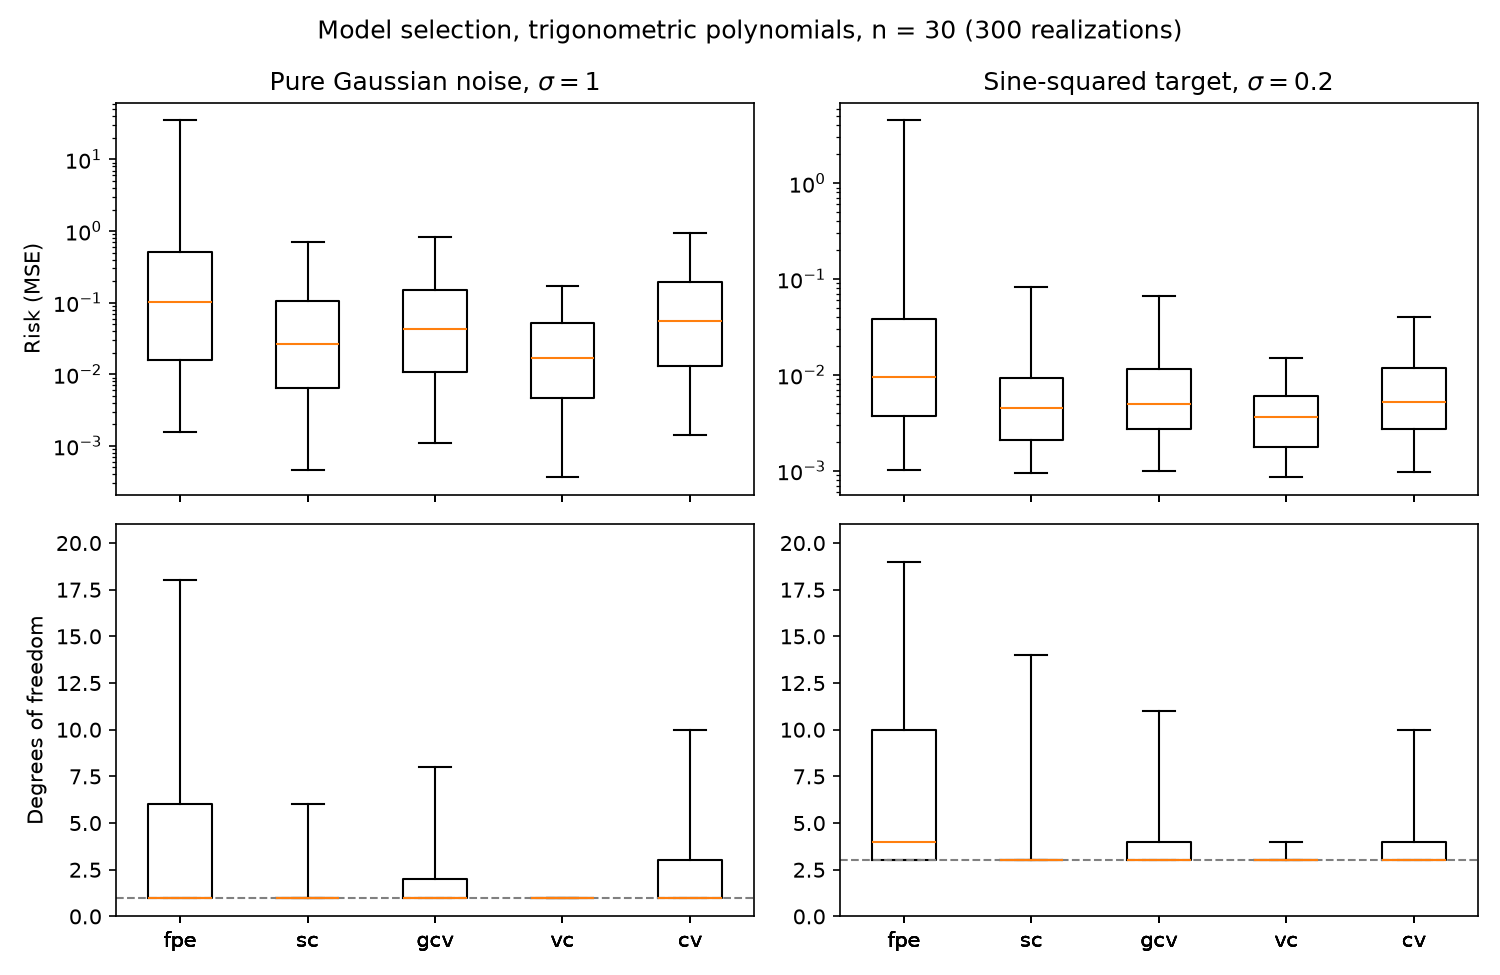
\includegraphics[width=0.92\linewidth]{p1_n30.png}
  \caption{Model selection results for $n = 30$ (300 realizations). Top: prediction risk (log scale);
           bottom: selected DoF. Left: pure noise; right: sine-squared.}
  \label{fig:p1n30}
\end{figure}

\begin{figure}[H]
  \centering
  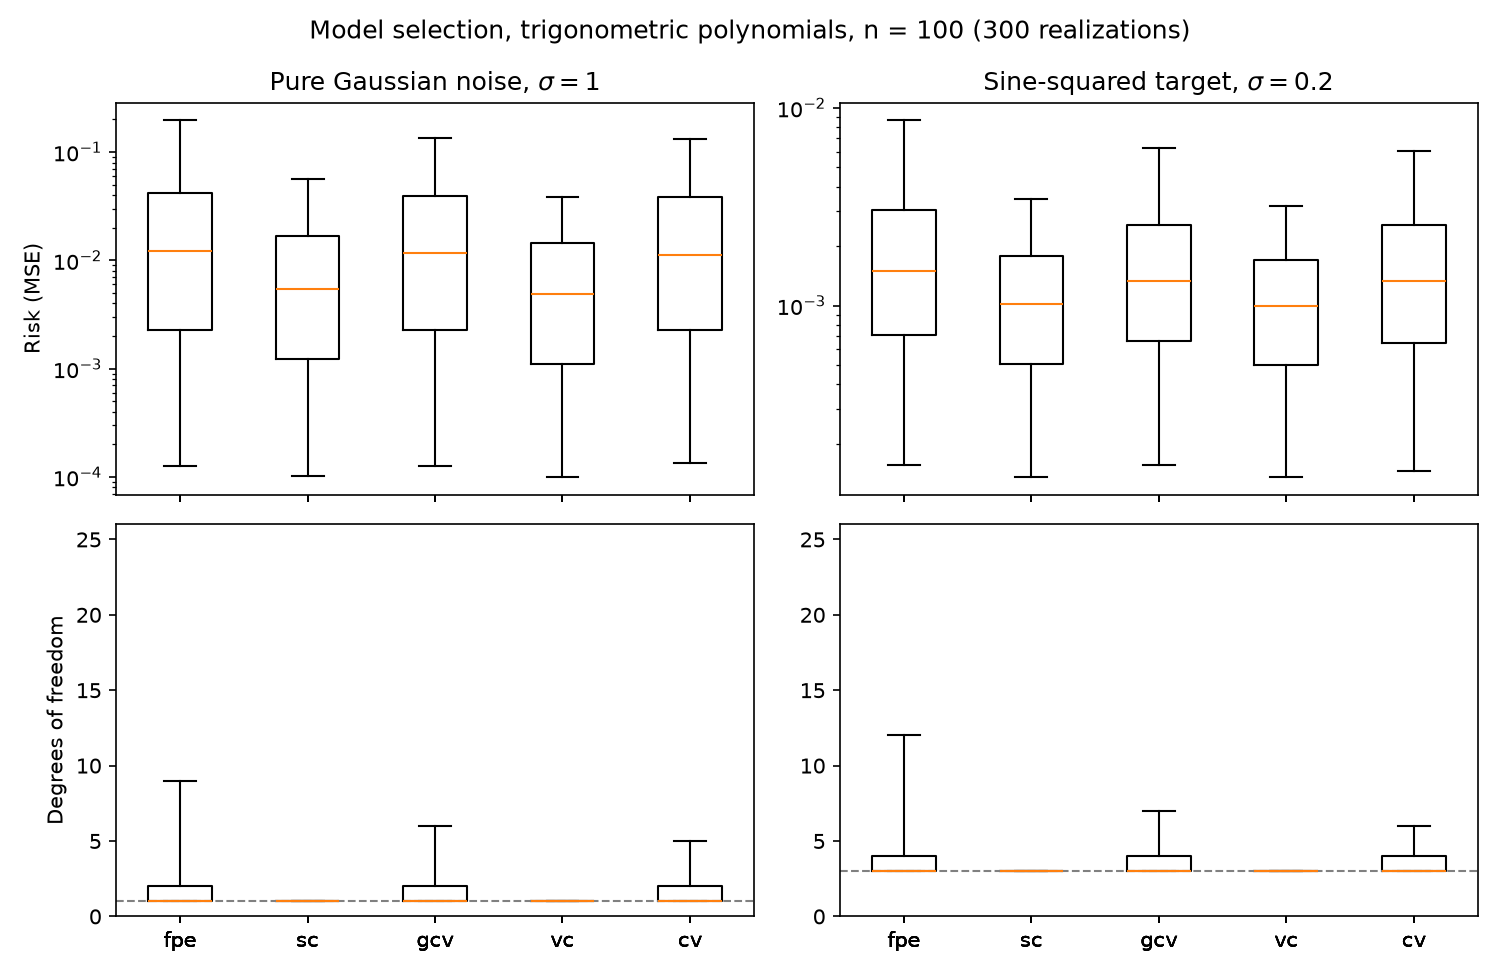
\includegraphics[width=0.92\linewidth]{p1_n100.png}
  \caption{Model selection results for $n = 100$ (300 realizations), same layout as Figure~\ref{fig:p1n30}.}
  \label{fig:p1n100}
\end{figure}

\begin{center}\small
\begin{tabular}{l rr rr rr rr}
\toprule
 & \multicolumn{4}{c}{$n = 30$} & \multicolumn{4}{c}{$n = 100$} \\
\cmidrule(lr){2-5}\cmidrule(lr){6-9}
 & \multicolumn{2}{c}{Pure noise} & \multicolumn{2}{c}{Sine-squared}
 & \multicolumn{2}{c}{Pure noise} & \multicolumn{2}{c}{Sine-squared} \\
Method & correct & risk p95 & correct & risk p95 & correct & risk p95 & correct & risk p95 \\
\midrule
fpe & 53.0\% & 35.7   & 46.3\% & 4.54   & 73.0\%  & 0.197  & 68.7\% & 0.0087 \\
sc  & 82.7\% & 0.708  & 76.0\% & 0.0821 & 95.3\%  & 0.0568 & 97.0\% & 0.0035 \\
gcv & 69.0\% & 0.831  & 67.7\% & 0.0672 & 74.0\%  & 0.134  & 73.0\% & 0.0063 \\
vc  & 97.7\% & 0.170  & 92.3\% & 0.0149 & 100.0\% & 0.0381 & 99.3\% & 0.0032 \\
cv  & 64.7\% & 0.945  & 64.7\% & 0.0402 & 74.7\%  & 0.132  & 74.3\% & 0.0060 \\
\bottomrule
\end{tabular}

\smallskip
\emph{correct}: share of the 300 realizations that selected the true DoF; \emph{risk p95}: 95th percentile of the prediction risk.
\end{center}

\paragraph{Small samples ($n = 30$).}
The share of correct selections follows the strength of the penalty: vc (97.7\% for pure noise, 92.3\% for
sine-squared) $>$ sc $>$ gcv $>$ cv $>$ fpe (53.0\%, 46.3\%). For sine-squared, fpe is the one method with a wrong
median DoF (4 instead of 3). Its light penalty lets a large drop in training error win: in one sine-squared sample,
fpe chose DoF $= 18$ while the other four methods chose DoF $= 3$. The tails of the risk distribution show the
largest gaps. For pure noise, the 95th-percentile risk of fpe (35.7) is about 200 times that of vc (0.17), while
their medians differ by a factor of six (0.103 vs.\ 0.017). In its worst 5\% of realizations, fpe picked models with
DoF 11--20, which swing far from zero between the training points; the worst vc selections had DoF 1 or 2.

\paragraph{Effect of sample size ($n = 100$).}
With $n = 100$, every method improves. vc selects the correct DoF in 100\% (pure noise) and 99.3\% (sine-squared) of
realizations, and sc in 95.3\% and 97.0\%. fpe, gcv, and cv level off at 70--75\%. For small $p$, these three
criteria charge about $2\sigma^2/n$ for each extra parameter, and a spurious term beats that charge with a probability
that does not shrink as $n$ grows. The sc charge, about $(\ln n)\,\sigma^2/n$, grows with $n$. The 95th-percentile
risk of fpe falls from 35.7 to 0.197 as its 95th-percentile DoF drops to 9 (pure noise) and 12 (sine-squared).

\subsection*{Conclusion}
Across both data sets and both sample sizes, the VC penalization chose the correct model most often and had the
lowest 95th-percentile risk. Its lead is widest at $n = 30$, where a wrong choice costs the most. The five methods
have similar median risks and separate in the worst 5\% of realizations, so a fair comparison needs the full risk
distribution.
.
% main.tex loads amsmath, graphicx, booktabs, float and sets
% \graphicspath{{../practice/}} (figures: p1_n30.png, p1_n100.png).
% All numbers come from HW2/practice/p1_mine.py (300 realizations, seed 0).
% ============================================================

\section*{Problem 1: Model selection for trigonometric polynomial regression}

\subsection*{Experimental setup}
I follow the procedure of Section~4.4 and compare analytic model selection criteria for univariate regression
with trigonometric polynomials
\[
  f_m(x) = w_0 + \sum_{k=1}^{m} w_k \cos(2\pi k x), \qquad \text{DoF} = m + 1,
\]
fitted by ordinary least squares. I draw inputs from $x \sim U[0,1]$ and use two data sets:
\begin{itemize}
  \item \textbf{Pure noise:} $y \sim N(0, 1)$. The true function is $f(x) = 0$, so the correct model is a constant (DoF $= 1$).
  \item \textbf{Sine-squared:} $y = \sin^2(2\pi x) + \varepsilon$, $\varepsilon \sim N(0, 0.2^2)$.
        Since $\sin^2(2\pi x) = \tfrac12 - \tfrac12\cos(4\pi x)$, the target belongs to the model with $m = 2$, and the correct DoF is 3.
\end{itemize}
I run 300 independent realizations for $n = 30$ (candidate DoF $1$--$20$) and $n = 100$ (candidate DoF $1$--$25$).
In each realization, every method selects a DoF. I refit the model with that DoF and measure its \emph{prediction
risk} as the mean squared error between the fitted model and the \emph{noise-free} target on 2000 independent test
points. No model can predict the noise, so this risk measures the distance between the selected model and the truth.

\subsection*{Model selection methods}
Training error falls as complexity grows, so it cannot guide model selection by itself. In one sine-squared sample
with $n = 30$, the training MSE fell from 0.107 at DoF $= 1$ to 0.0067 at DoF $= 20$, below the noise variance
$\sigma^2 = 0.04$. Each analytic method multiplies the training error $R_{\text{emp}}$ by a penalization factor
$r(p)$, where $p = \text{DoF}/n$, and selects the DoF that minimizes $r(p)\,R_{\text{emp}}$:
\begin{center}\small
\begin{tabular}{lll}
\toprule
Method & Penalization factor $r(p)$ & Reference \\
\midrule
Final prediction error (fpe) & $(1+p)/(1-p)$ & Eq.~(2.11) \\
Schwartz criterion (sc) & $1 + (\ln n)\, p/(1-p)$ & Eq.~(2.12) \\
Generalized cross-validation (gcv) & $(1-p)^{-2}$ & Eq.~(2.13) \\
VC bound (vc) & $\bigl(1 - \sqrt{p - p\ln p + \ln n/(2n)}\bigr)_+^{-1}$ & Eq.~(4.15) \\
\bottomrule
\end{tabular}
\end{center}
For vc, I set the factor to infinity when the term under the square root reaches 1, which excludes that model.
At $p = 0.1$ the four factors lie between 1.2 and 1.5. At $p = 0.5$ with $n = 30$ they spread out: fpe gives 3.0,
gcv 4.0, sc 4.4, and vc 20.2.

The fifth method, leave-one-out cross-validation (cv), estimates prediction risk from held-out data. I compute the
leave-one-out error from a single fit with the leverage formula $e_i/(1 - h_{ii})$, where $e_i$ is the ordinary
residual and $h_{ii}$ the $i$-th diagonal entry of the hat matrix. In my checks it matched the result of $n$
explicit refits to four decimal places.

\subsection*{Results}
Figures~\ref{fig:p1n30} and~\ref{fig:p1n100} present the results in the style of Figs.~4.10--4.11. Each box spans
the 25th to 75th percentiles with a line at the median, and the whiskers reach the 5th and 95th percentiles. The risk
panels use a logarithmic scale, and a dashed line in the DoF panels marks the correct DoF.

\begin{figure}[H]
  \centering
  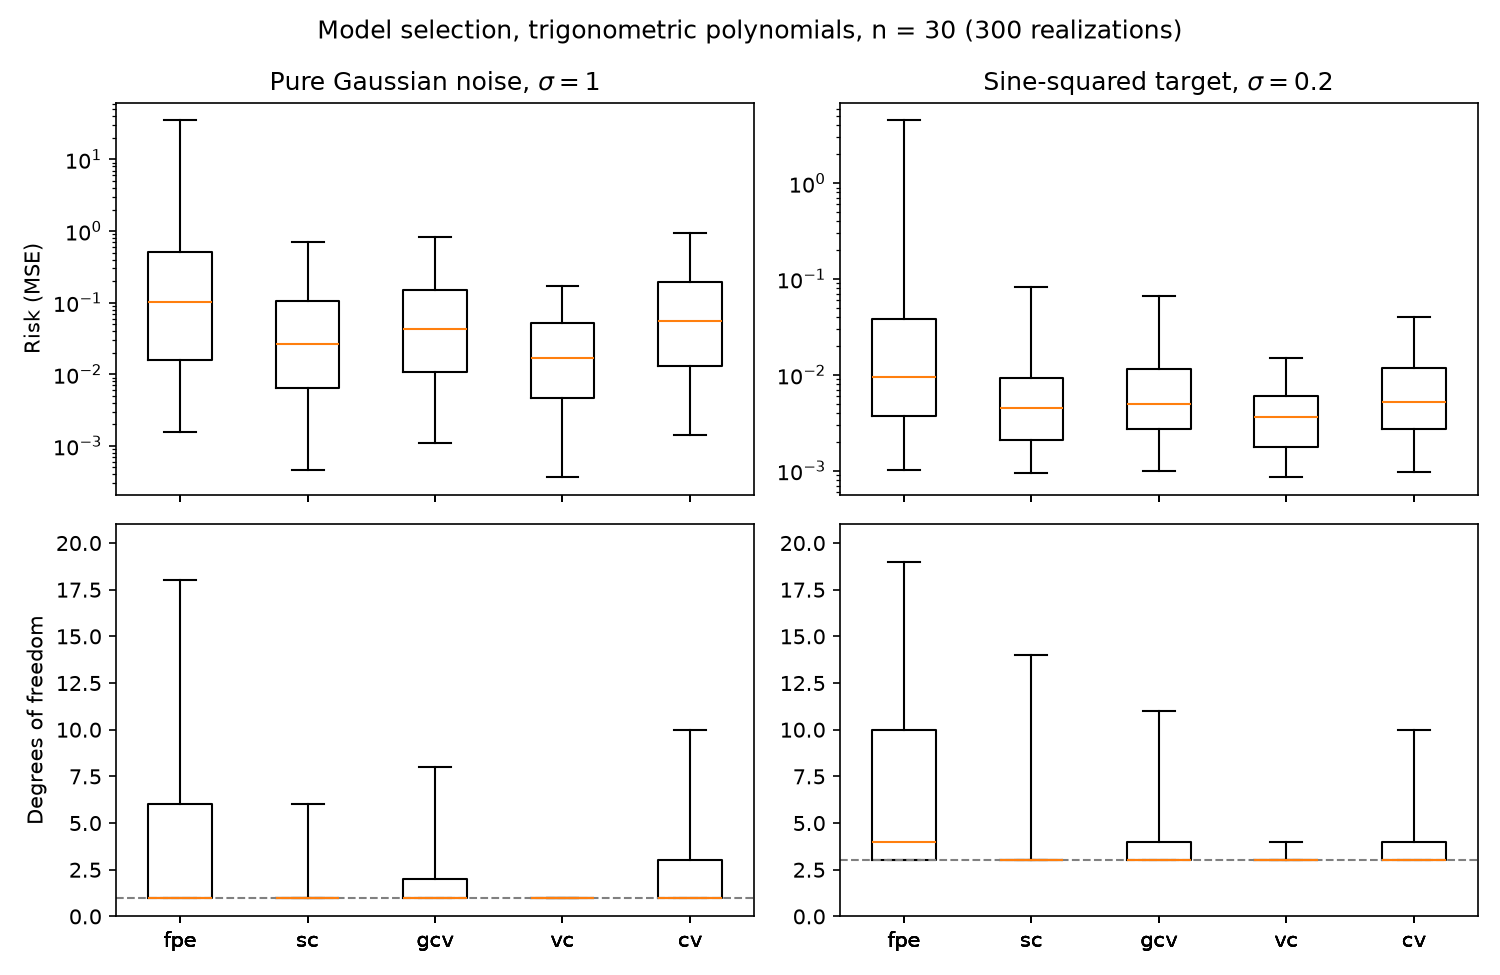
\includegraphics[width=0.92\linewidth]{p1_n30.png}
  \caption{Model selection results for $n = 30$ (300 realizations). Top: prediction risk (log scale);
           bottom: selected DoF. Left: pure noise; right: sine-squared.}
  \label{fig:p1n30}
\end{figure}

\begin{figure}[H]
  \centering
  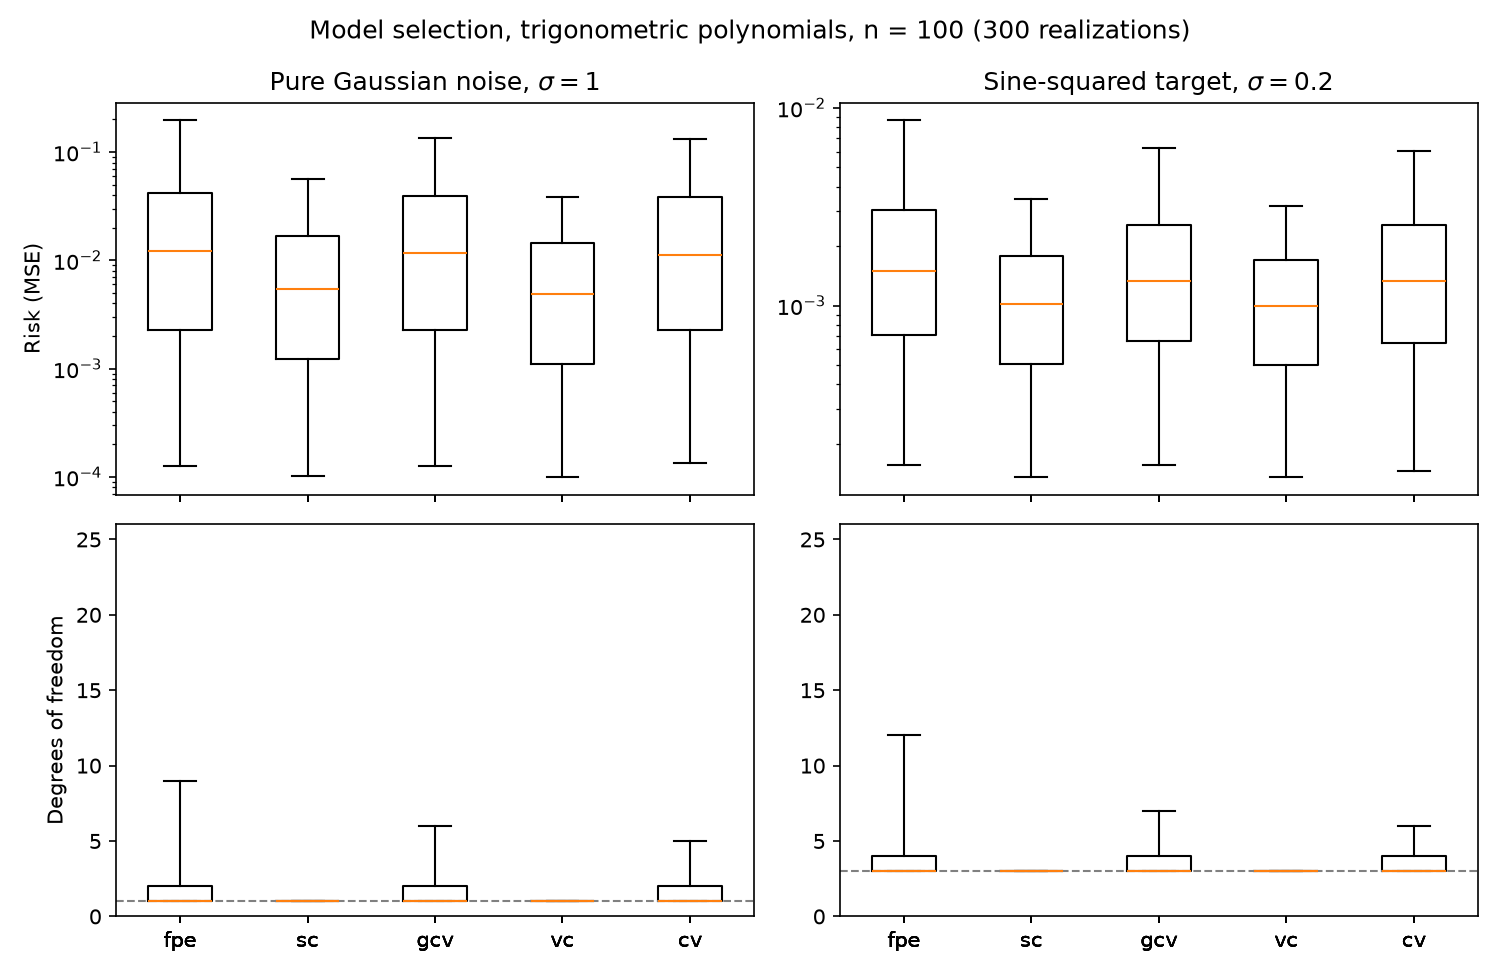
\includegraphics[width=0.92\linewidth]{p1_n100.png}
  \caption{Model selection results for $n = 100$ (300 realizations), same layout as Figure~\ref{fig:p1n30}.}
  \label{fig:p1n100}
\end{figure}

\begin{center}\small
\begin{tabular}{l rr rr rr rr}
\toprule
 & \multicolumn{4}{c}{$n = 30$} & \multicolumn{4}{c}{$n = 100$} \\
\cmidrule(lr){2-5}\cmidrule(lr){6-9}
 & \multicolumn{2}{c}{Pure noise} & \multicolumn{2}{c}{Sine-squared}
 & \multicolumn{2}{c}{Pure noise} & \multicolumn{2}{c}{Sine-squared} \\
Method & correct & risk p95 & correct & risk p95 & correct & risk p95 & correct & risk p95 \\
\midrule
fpe & 53.0\% & 35.7   & 46.3\% & 4.54   & 73.0\%  & 0.197  & 68.7\% & 0.0087 \\
sc  & 82.7\% & 0.708  & 76.0\% & 0.0821 & 95.3\%  & 0.0568 & 97.0\% & 0.0035 \\
gcv & 69.0\% & 0.831  & 67.7\% & 0.0672 & 74.0\%  & 0.134  & 73.0\% & 0.0063 \\
vc  & 97.7\% & 0.170  & 92.3\% & 0.0149 & 100.0\% & 0.0381 & 99.3\% & 0.0032 \\
cv  & 64.7\% & 0.945  & 64.7\% & 0.0402 & 74.7\%  & 0.132  & 74.3\% & 0.0060 \\
\bottomrule
\end{tabular}

\smallskip
\emph{correct}: share of the 300 realizations that selected the true DoF; \emph{risk p95}: 95th percentile of the prediction risk.
\end{center}

\paragraph{Small samples ($n = 30$).}
The share of correct selections follows the strength of the penalty: vc (97.7\% for pure noise, 92.3\% for
sine-squared) $>$ sc $>$ gcv $>$ cv $>$ fpe (53.0\%, 46.3\%). For sine-squared, fpe is the one method with a wrong
median DoF (4 instead of 3). Its light penalty lets a large drop in training error win: in one sine-squared sample,
fpe chose DoF $= 18$ while the other four methods chose DoF $= 3$. The tails of the risk distribution show the
largest gaps. For pure noise, the 95th-percentile risk of fpe (35.7) is about 200 times that of vc (0.17), while
their medians differ by a factor of six (0.103 vs.\ 0.017). In its worst 5\% of realizations, fpe picked models with
DoF 11--20, which swing far from zero between the training points; the worst vc selections had DoF 1 or 2.

\paragraph{Effect of sample size ($n = 100$).}
With $n = 100$, every method improves. vc selects the correct DoF in 100\% (pure noise) and 99.3\% (sine-squared) of
realizations, and sc in 95.3\% and 97.0\%. fpe, gcv, and cv level off at 70--75\%. For small $p$, these three
criteria charge about $2\sigma^2/n$ for each extra parameter, and a spurious term beats that charge with a probability
that does not shrink as $n$ grows. The sc charge, about $(\ln n)\,\sigma^2/n$, grows with $n$. The 95th-percentile
risk of fpe falls from 35.7 to 0.197 as its 95th-percentile DoF drops to 9 (pure noise) and 12 (sine-squared).

\subsection*{Conclusion}
Across both data sets and both sample sizes, the VC penalization chose the correct model most often and had the
lowest 95th-percentile risk. Its lead is widest at $n = 30$, where a wrong choice costs the most. The five methods
have similar median risks and separate in the worst 5\% of realizations, so a fair comparison needs the full risk
distribution.
.
% main.tex loads amsmath, graphicx, booktabs, float and sets
% \graphicspath{{../practice/}} (figures: p1_n30.png, p1_n100.png).
% All numbers come from HW2/practice/p1_mine.py (300 realizations, seed 0).
% ============================================================

\section*{Problem 1: Model selection for trigonometric polynomial regression}

\subsection*{Experimental setup}
I follow the procedure of Section~4.4 and compare analytic model selection criteria for univariate regression
with trigonometric polynomials
\[
  f_m(x) = w_0 + \sum_{k=1}^{m} w_k \cos(2\pi k x), \qquad \text{DoF} = m + 1,
\]
fitted by ordinary least squares. I draw inputs from $x \sim U[0,1]$ and use two data sets:
\begin{itemize}
  \item \textbf{Pure noise:} $y \sim N(0, 1)$. The true function is $f(x) = 0$, so the correct model is a constant (DoF $= 1$).
  \item \textbf{Sine-squared:} $y = \sin^2(2\pi x) + \varepsilon$, $\varepsilon \sim N(0, 0.2^2)$.
        Since $\sin^2(2\pi x) = \tfrac12 - \tfrac12\cos(4\pi x)$, the target belongs to the model with $m = 2$, and the correct DoF is 3.
\end{itemize}
I run 300 independent realizations for $n = 30$ (candidate DoF $1$--$20$) and $n = 100$ (candidate DoF $1$--$25$).
In each realization, every method selects a DoF. I refit the model with that DoF and measure its \emph{prediction
risk} as the mean squared error between the fitted model and the \emph{noise-free} target on 2000 independent test
points. No model can predict the noise, so this risk measures the distance between the selected model and the truth.

\subsection*{Model selection methods}
Training error falls as complexity grows, so it cannot guide model selection by itself. In one sine-squared sample
with $n = 30$, the training MSE fell from 0.107 at DoF $= 1$ to 0.0067 at DoF $= 20$, below the noise variance
$\sigma^2 = 0.04$. Each analytic method multiplies the training error $R_{\text{emp}}$ by a penalization factor
$r(p)$, where $p = \text{DoF}/n$, and selects the DoF that minimizes $r(p)\,R_{\text{emp}}$:
\begin{center}\small
\begin{tabular}{lll}
\toprule
Method & Penalization factor $r(p)$ & Reference \\
\midrule
Final prediction error (fpe) & $(1+p)/(1-p)$ & Eq.~(2.11) \\
Schwartz criterion (sc) & $1 + (\ln n)\, p/(1-p)$ & Eq.~(2.12) \\
Generalized cross-validation (gcv) & $(1-p)^{-2}$ & Eq.~(2.13) \\
VC bound (vc) & $\bigl(1 - \sqrt{p - p\ln p + \ln n/(2n)}\bigr)_+^{-1}$ & Eq.~(4.15) \\
\bottomrule
\end{tabular}
\end{center}
For vc, I set the factor to infinity when the term under the square root reaches 1, which excludes that model.
At $p = 0.1$ the four factors lie between 1.2 and 1.5. At $p = 0.5$ with $n = 30$ they spread out: fpe gives 3.0,
gcv 4.0, sc 4.4, and vc 20.2.

The fifth method, leave-one-out cross-validation (cv), estimates prediction risk from held-out data. I compute the
leave-one-out error from a single fit with the leverage formula $e_i/(1 - h_{ii})$, where $e_i$ is the ordinary
residual and $h_{ii}$ the $i$-th diagonal entry of the hat matrix. In my checks it matched the result of $n$
explicit refits to four decimal places.

\subsection*{Results}
Figures~\ref{fig:p1n30} and~\ref{fig:p1n100} present the results in the style of Figs.~4.10--4.11. Each box spans
the 25th to 75th percentiles with a line at the median, and the whiskers reach the 5th and 95th percentiles. The risk
panels use a logarithmic scale, and a dashed line in the DoF panels marks the correct DoF.

\begin{figure}[H]
  \centering
  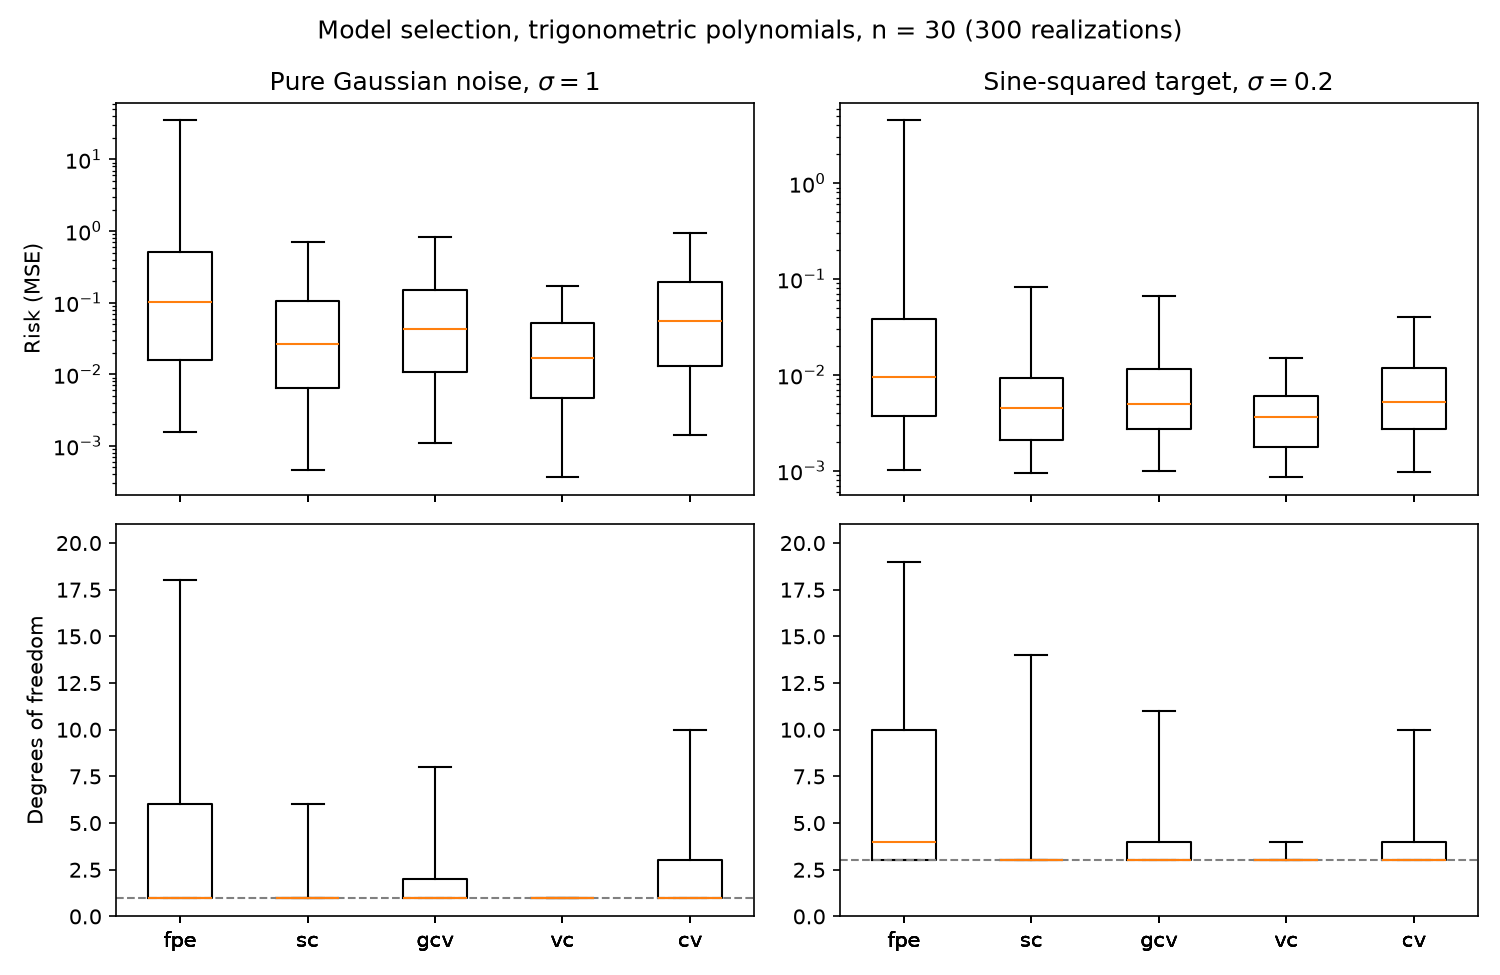
\includegraphics[width=0.92\linewidth]{p1_n30.png}
  \caption{Model selection results for $n = 30$ (300 realizations). Top: prediction risk (log scale);
           bottom: selected DoF. Left: pure noise; right: sine-squared.}
  \label{fig:p1n30}
\end{figure}

\begin{figure}[H]
  \centering
  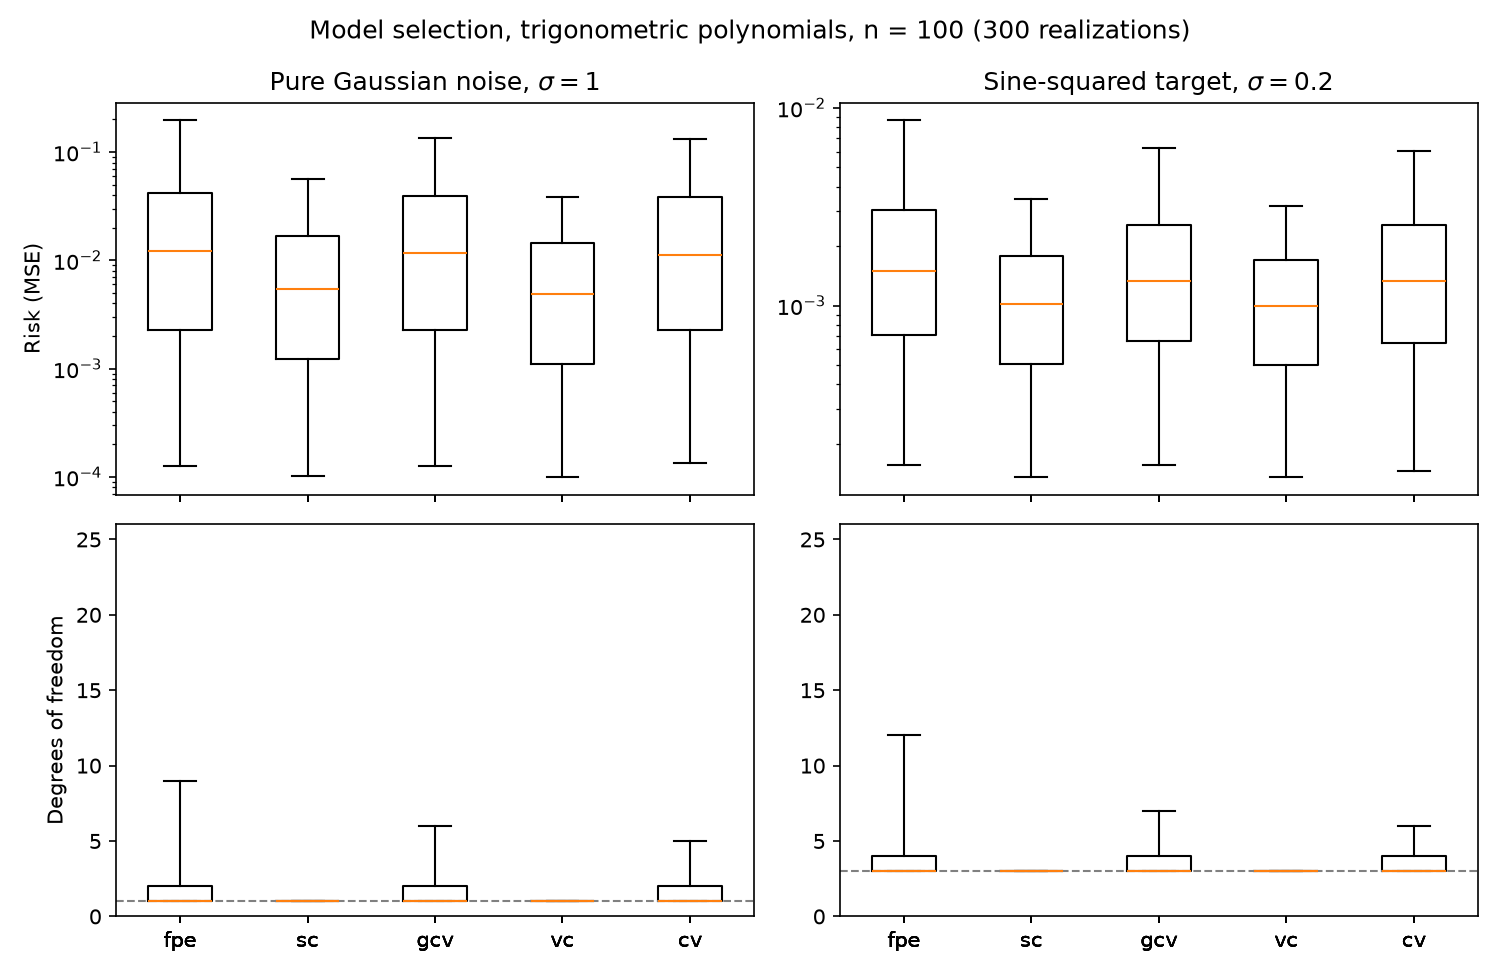
\includegraphics[width=0.92\linewidth]{p1_n100.png}
  \caption{Model selection results for $n = 100$ (300 realizations), same layout as Figure~\ref{fig:p1n30}.}
  \label{fig:p1n100}
\end{figure}

\begin{center}\small
\begin{tabular}{l rr rr rr rr}
\toprule
 & \multicolumn{4}{c}{$n = 30$} & \multicolumn{4}{c}{$n = 100$} \\
\cmidrule(lr){2-5}\cmidrule(lr){6-9}
 & \multicolumn{2}{c}{Pure noise} & \multicolumn{2}{c}{Sine-squared}
 & \multicolumn{2}{c}{Pure noise} & \multicolumn{2}{c}{Sine-squared} \\
Method & correct & risk p95 & correct & risk p95 & correct & risk p95 & correct & risk p95 \\
\midrule
fpe & 53.0\% & 35.7   & 46.3\% & 4.54   & 73.0\%  & 0.197  & 68.7\% & 0.0087 \\
sc  & 82.7\% & 0.708  & 76.0\% & 0.0821 & 95.3\%  & 0.0568 & 97.0\% & 0.0035 \\
gcv & 69.0\% & 0.831  & 67.7\% & 0.0672 & 74.0\%  & 0.134  & 73.0\% & 0.0063 \\
vc  & 97.7\% & 0.170  & 92.3\% & 0.0149 & 100.0\% & 0.0381 & 99.3\% & 0.0032 \\
cv  & 64.7\% & 0.945  & 64.7\% & 0.0402 & 74.7\%  & 0.132  & 74.3\% & 0.0060 \\
\bottomrule
\end{tabular}

\smallskip
\emph{correct}: share of the 300 realizations that selected the true DoF; \emph{risk p95}: 95th percentile of the prediction risk.
\end{center}

\paragraph{Small samples ($n = 30$).}
The share of correct selections follows the strength of the penalty: vc (97.7\% for pure noise, 92.3\% for
sine-squared) $>$ sc $>$ gcv $>$ cv $>$ fpe (53.0\%, 46.3\%). For sine-squared, fpe is the one method with a wrong
median DoF (4 instead of 3). Its light penalty lets a large drop in training error win: in one sine-squared sample,
fpe chose DoF $= 18$ while the other four methods chose DoF $= 3$. The tails of the risk distribution show the
largest gaps. For pure noise, the 95th-percentile risk of fpe (35.7) is about 200 times that of vc (0.17), while
their medians differ by a factor of six (0.103 vs.\ 0.017). In its worst 5\% of realizations, fpe picked models with
DoF 11--20, which swing far from zero between the training points; the worst vc selections had DoF 1 or 2.

\paragraph{Effect of sample size ($n = 100$).}
With $n = 100$, every method improves. vc selects the correct DoF in 100\% (pure noise) and 99.3\% (sine-squared) of
realizations, and sc in 95.3\% and 97.0\%. fpe, gcv, and cv level off at 70--75\%. For small $p$, these three
criteria charge about $2\sigma^2/n$ for each extra parameter, and a spurious term beats that charge with a probability
that does not shrink as $n$ grows. The sc charge, about $(\ln n)\,\sigma^2/n$, grows with $n$. The 95th-percentile
risk of fpe falls from 35.7 to 0.197 as its 95th-percentile DoF drops to 9 (pure noise) and 12 (sine-squared).

\subsection*{Conclusion}
Across both data sets and both sample sizes, the VC penalization chose the correct model most often and had the
lowest 95th-percentile risk. Its lead is widest at $n = 30$, where a wrong choice costs the most. The five methods
have similar median risks and separate in the worst 5\% of realizations, so a fair comparison needs the full risk
distribution.
.
% main.tex loads amsmath, graphicx, booktabs, float and sets
% \graphicspath{{../practice/}} (figures: p1_n30.png, p1_n100.png).
% All numbers come from HW2/practice/p1_mine.py (300 realizations, seed 0).
% ============================================================

\section*{Problem 1: Model selection for trigonometric polynomial regression}

\subsection*{Experimental setup}
I follow the procedure of Section~4.4 and compare analytic model selection criteria for univariate regression
with trigonometric polynomials
\[
  f_m(x) = w_0 + \sum_{k=1}^{m} w_k \cos(2\pi k x), \qquad \text{DoF} = m + 1,
\]
fitted by ordinary least squares. I draw inputs from $x \sim U[0,1]$ and use two data sets:
\begin{itemize}
  \item \textbf{Pure noise:} $y \sim N(0, 1)$. The true function is $f(x) = 0$, so the correct model is a constant (DoF $= 1$).
  \item \textbf{Sine-squared:} $y = \sin^2(2\pi x) + \varepsilon$, $\varepsilon \sim N(0, 0.2^2)$.
        Since $\sin^2(2\pi x) = \tfrac12 - \tfrac12\cos(4\pi x)$, the target belongs to the model with $m = 2$, and the correct DoF is 3.
\end{itemize}
I run 300 independent realizations for $n = 30$ (candidate DoF $1$--$20$) and $n = 100$ (candidate DoF $1$--$25$).
In each realization, every method selects a DoF. I refit the model with that DoF and measure its \emph{prediction
risk} as the mean squared error between the fitted model and the \emph{noise-free} target on 2000 independent test
points. No model can predict the noise, so this risk measures the distance between the selected model and the truth.

\subsection*{Model selection methods}
Training error falls as complexity grows, so it cannot guide model selection by itself. In one sine-squared sample
with $n = 30$, the training MSE fell from 0.107 at DoF $= 1$ to 0.0067 at DoF $= 20$, below the noise variance
$\sigma^2 = 0.04$. Each analytic method multiplies the training error $R_{\text{emp}}$ by a penalization factor
$r(p)$, where $p = \text{DoF}/n$, and selects the DoF that minimizes $r(p)\,R_{\text{emp}}$:
\begin{center}\small
\begin{tabular}{lll}
\toprule
Method & Penalization factor $r(p)$ & Reference \\
\midrule
Final prediction error (fpe) & $(1+p)/(1-p)$ & Eq.~(2.11) \\
Schwartz criterion (sc) & $1 + (\ln n)\, p/(1-p)$ & Eq.~(2.12) \\
Generalized cross-validation (gcv) & $(1-p)^{-2}$ & Eq.~(2.13) \\
VC bound (vc) & $\bigl(1 - \sqrt{p - p\ln p + \ln n/(2n)}\bigr)_+^{-1}$ & Eq.~(4.15) \\
\bottomrule
\end{tabular}
\end{center}
For vc, I set the factor to infinity when the term under the square root reaches 1, which excludes that model.
At $p = 0.1$ the four factors lie between 1.2 and 1.5. At $p = 0.5$ with $n = 30$ they spread out: fpe gives 3.0,
gcv 4.0, sc 4.4, and vc 20.2.

The fifth method, leave-one-out cross-validation (cv), estimates prediction risk from held-out data. I compute the
leave-one-out error from a single fit with the leverage formula $e_i/(1 - h_{ii})$, where $e_i$ is the ordinary
residual and $h_{ii}$ the $i$-th diagonal entry of the hat matrix. In my checks it matched the result of $n$
explicit refits to four decimal places.

\subsection*{Results}
Figures~\ref{fig:p1n30} and~\ref{fig:p1n100} present the results in the style of Figs.~4.10--4.11. Each box spans
the 25th to 75th percentiles with a line at the median, and the whiskers reach the 5th and 95th percentiles. The risk
panels use a logarithmic scale, and a dashed line in the DoF panels marks the correct DoF.

\begin{figure}[H]
  \centering
  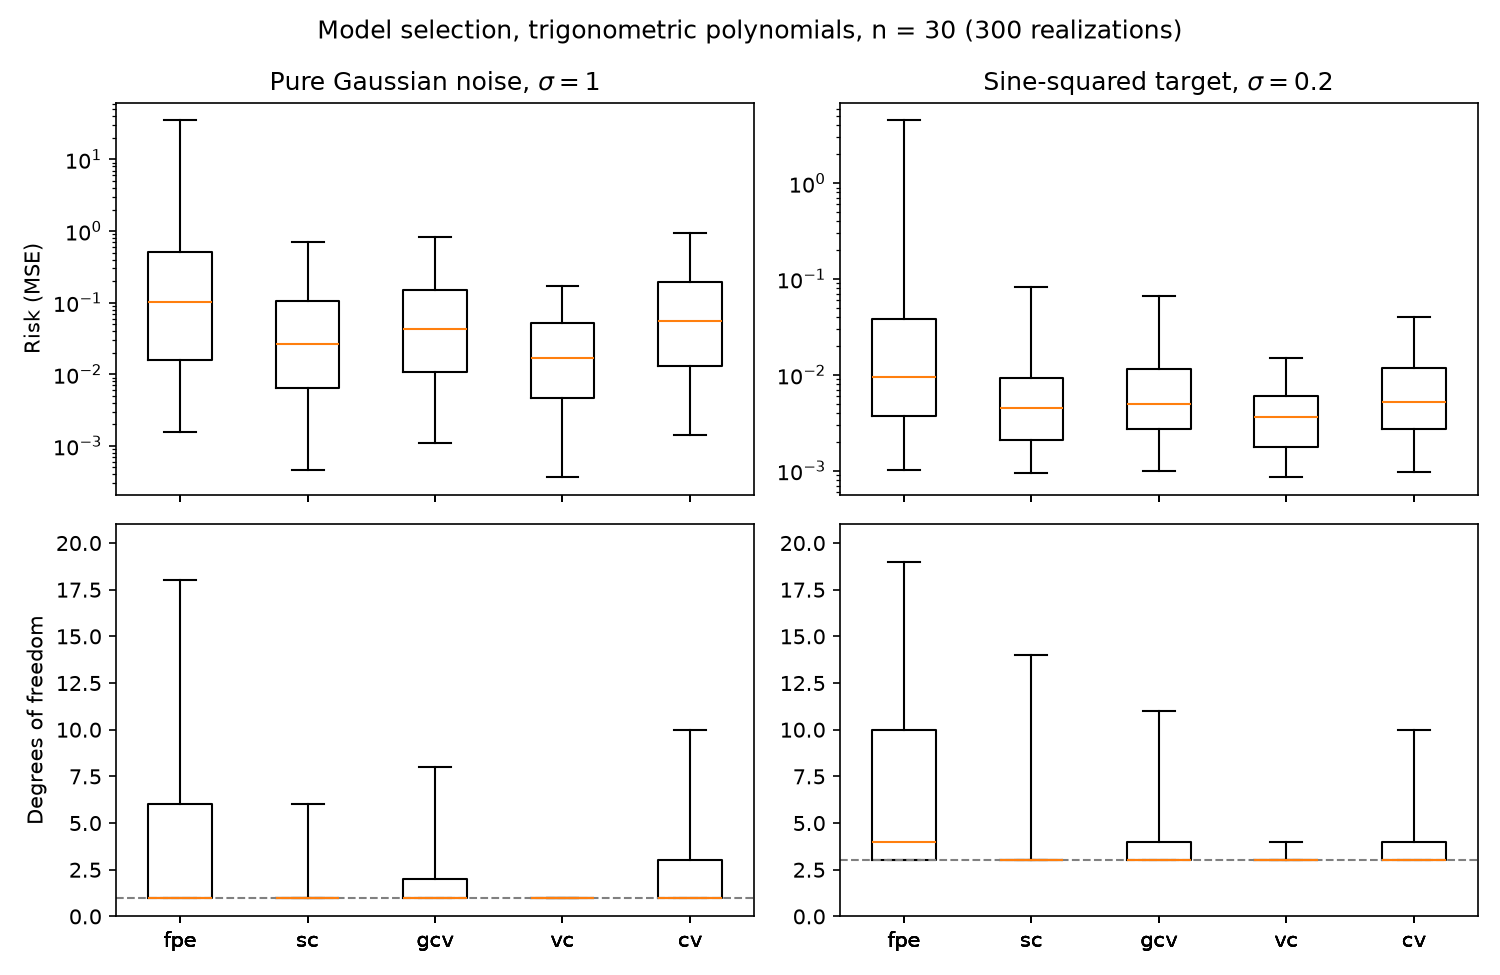
\includegraphics[width=0.92\linewidth]{p1_n30.png}
  \caption{Model selection results for $n = 30$ (300 realizations). Top: prediction risk (log scale);
           bottom: selected DoF. Left: pure noise; right: sine-squared.}
  \label{fig:p1n30}
\end{figure}

\begin{figure}[H]
  \centering
  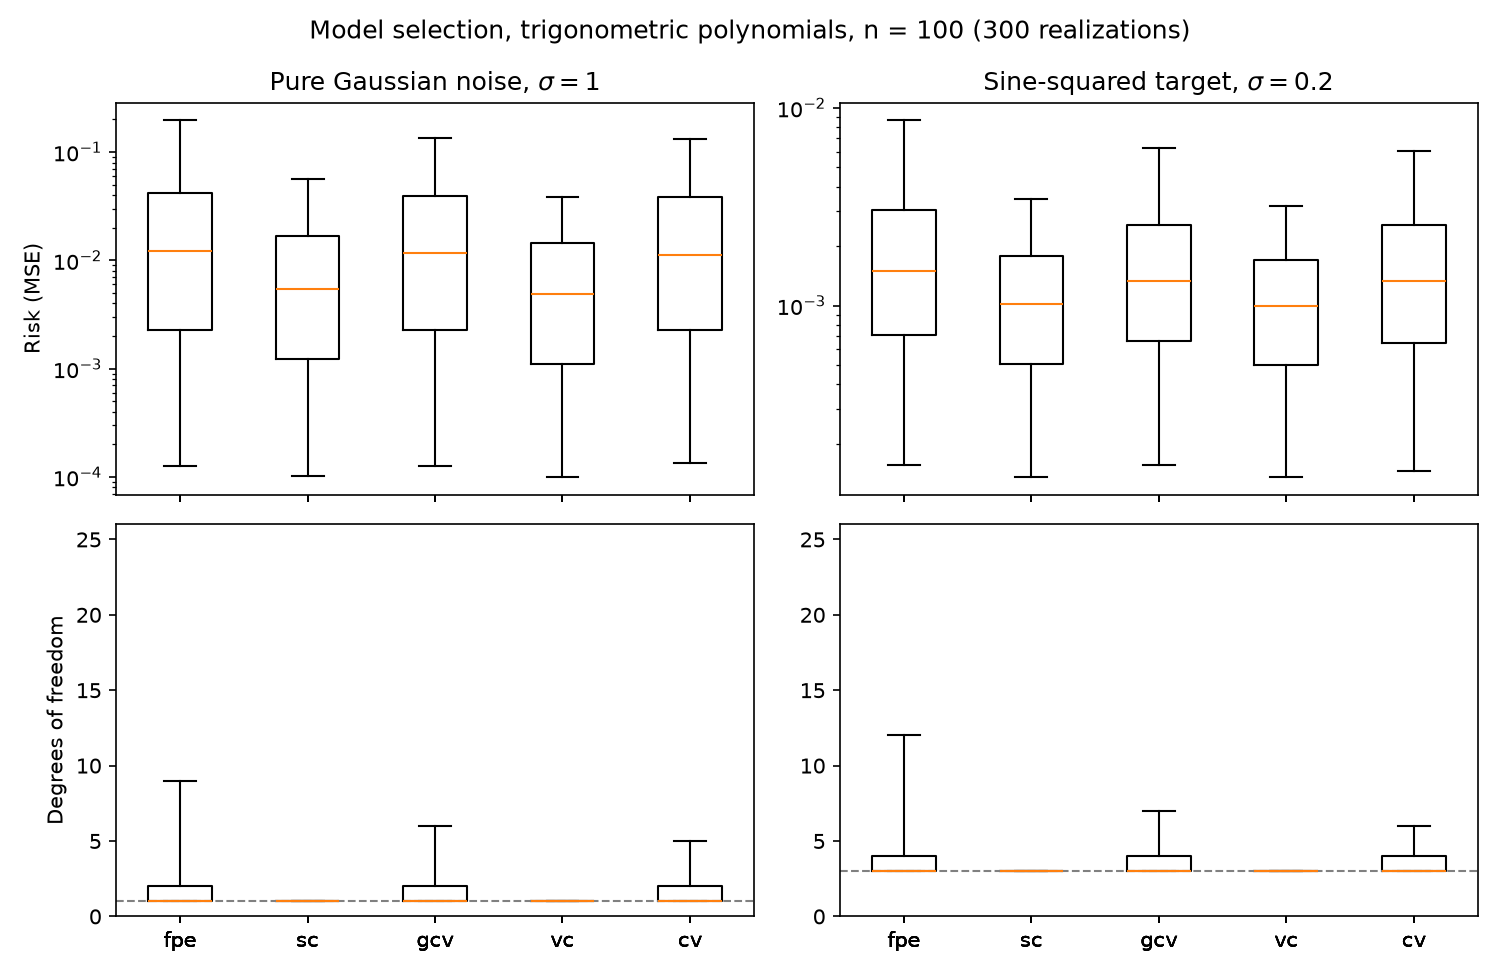
\includegraphics[width=0.92\linewidth]{p1_n100.png}
  \caption{Model selection results for $n = 100$ (300 realizations), same layout as Figure~\ref{fig:p1n30}.}
  \label{fig:p1n100}
\end{figure}

\begin{center}\small
\begin{tabular}{l rr rr rr rr}
\toprule
 & \multicolumn{4}{c}{$n = 30$} & \multicolumn{4}{c}{$n = 100$} \\
\cmidrule(lr){2-5}\cmidrule(lr){6-9}
 & \multicolumn{2}{c}{Pure noise} & \multicolumn{2}{c}{Sine-squared}
 & \multicolumn{2}{c}{Pure noise} & \multicolumn{2}{c}{Sine-squared} \\
Method & correct & risk p95 & correct & risk p95 & correct & risk p95 & correct & risk p95 \\
\midrule
fpe & 53.0\% & 35.7   & 46.3\% & 4.54   & 73.0\%  & 0.197  & 68.7\% & 0.0087 \\
sc  & 82.7\% & 0.708  & 76.0\% & 0.0821 & 95.3\%  & 0.0568 & 97.0\% & 0.0035 \\
gcv & 69.0\% & 0.831  & 67.7\% & 0.0672 & 74.0\%  & 0.134  & 73.0\% & 0.0063 \\
vc  & 97.7\% & 0.170  & 92.3\% & 0.0149 & 100.0\% & 0.0381 & 99.3\% & 0.0032 \\
cv  & 64.7\% & 0.945  & 64.7\% & 0.0402 & 74.7\%  & 0.132  & 74.3\% & 0.0060 \\
\bottomrule
\end{tabular}

\smallskip
\emph{correct}: share of the 300 realizations that selected the true DoF; \emph{risk p95}: 95th percentile of the prediction risk.
\end{center}

\paragraph{Small samples ($n = 30$).}
The share of correct selections follows the strength of the penalty: vc (97.7\% for pure noise, 92.3\% for
sine-squared) $>$ sc $>$ gcv $>$ cv $>$ fpe (53.0\%, 46.3\%). For sine-squared, fpe is the one method with a wrong
median DoF (4 instead of 3). Its light penalty lets a large drop in training error win: in one sine-squared sample,
fpe chose DoF $= 18$ while the other four methods chose DoF $= 3$. The tails of the risk distribution show the
largest gaps. For pure noise, the 95th-percentile risk of fpe (35.7) is about 200 times that of vc (0.17), while
their medians differ by a factor of six (0.103 vs.\ 0.017). In its worst 5\% of realizations, fpe picked models with
DoF 11--20, which swing far from zero between the training points; the worst vc selections had DoF 1 or 2.

\paragraph{Effect of sample size ($n = 100$).}
With $n = 100$, every method improves. vc selects the correct DoF in 100\% (pure noise) and 99.3\% (sine-squared) of
realizations, and sc in 95.3\% and 97.0\%. fpe, gcv, and cv level off at 70--75\%. For small $p$, these three
criteria charge about $2\sigma^2/n$ for each extra parameter, and a spurious term beats that charge with a probability
that does not shrink as $n$ grows. The sc charge, about $(\ln n)\,\sigma^2/n$, grows with $n$. The 95th-percentile
risk of fpe falls from 35.7 to 0.197 as its 95th-percentile DoF drops to 9 (pure noise) and 12 (sine-squared).

\subsection*{Conclusion}
Across both data sets and both sample sizes, the VC penalization chose the correct model most often and had the
lowest 95th-percentile risk. Its lead is widest at $n = 30$, where a wrong choice costs the most. The five methods
have similar median risks and separate in the worst 5\% of realizations, so a fair comparison needs the full risk
distribution.
